% Options for packages loaded elsewhere
\PassOptionsToPackage{unicode}{hyperref}
\PassOptionsToPackage{hyphens}{url}
%
\documentclass[
  man]{apa6}
\usepackage{amsmath,amssymb}
\usepackage{iftex}
\ifPDFTeX
  \usepackage[T1]{fontenc}
  \usepackage[utf8]{inputenc}
  \usepackage{textcomp} % provide euro and other symbols
\else % if luatex or xetex
  \usepackage{unicode-math} % this also loads fontspec
  \defaultfontfeatures{Scale=MatchLowercase}
  \defaultfontfeatures[\rmfamily]{Ligatures=TeX,Scale=1}
\fi
\usepackage{lmodern}
\ifPDFTeX\else
  % xetex/luatex font selection
\fi
% Use upquote if available, for straight quotes in verbatim environments
\IfFileExists{upquote.sty}{\usepackage{upquote}}{}
\IfFileExists{microtype.sty}{% use microtype if available
  \usepackage[]{microtype}
  \UseMicrotypeSet[protrusion]{basicmath} % disable protrusion for tt fonts
}{}
\makeatletter
\@ifundefined{KOMAClassName}{% if non-KOMA class
  \IfFileExists{parskip.sty}{%
    \usepackage{parskip}
  }{% else
    \setlength{\parindent}{0pt}
    \setlength{\parskip}{6pt plus 2pt minus 1pt}}
}{% if KOMA class
  \KOMAoptions{parskip=half}}
\makeatother
\usepackage{xcolor}
\usepackage{graphicx}
\makeatletter
\newsavebox\pandoc@box
\newcommand*\pandocbounded[1]{% scales image to fit in text height/width
  \sbox\pandoc@box{#1}%
  \Gscale@div\@tempa{\textheight}{\dimexpr\ht\pandoc@box+\dp\pandoc@box\relax}%
  \Gscale@div\@tempb{\linewidth}{\wd\pandoc@box}%
  \ifdim\@tempb\p@<\@tempa\p@\let\@tempa\@tempb\fi% select the smaller of both
  \ifdim\@tempa\p@<\p@\scalebox{\@tempa}{\usebox\pandoc@box}%
  \else\usebox{\pandoc@box}%
  \fi%
}
% Set default figure placement to htbp
\def\fps@figure{htbp}
\makeatother
\setlength{\emergencystretch}{3em} % prevent overfull lines
\providecommand{\tightlist}{%
  \setlength{\itemsep}{0pt}\setlength{\parskip}{0pt}}
\setcounter{secnumdepth}{-\maxdimen} % remove section numbering
% Make \paragraph and \subparagraph free-standing
\makeatletter
\ifx\paragraph\undefined\else
  \let\oldparagraph\paragraph
  \renewcommand{\paragraph}{
    \@ifstar
      \xxxParagraphStar
      \xxxParagraphNoStar
  }
  \newcommand{\xxxParagraphStar}[1]{\oldparagraph*{#1}\mbox{}}
  \newcommand{\xxxParagraphNoStar}[1]{\oldparagraph{#1}\mbox{}}
\fi
\ifx\subparagraph\undefined\else
  \let\oldsubparagraph\subparagraph
  \renewcommand{\subparagraph}{
    \@ifstar
      \xxxSubParagraphStar
      \xxxSubParagraphNoStar
  }
  \newcommand{\xxxSubParagraphStar}[1]{\oldsubparagraph*{#1}\mbox{}}
  \newcommand{\xxxSubParagraphNoStar}[1]{\oldsubparagraph{#1}\mbox{}}
\fi
\makeatother
% definitions for citeproc citations
\NewDocumentCommand\citeproctext{}{}
\NewDocumentCommand\citeproc{mm}{%
  \begingroup\def\citeproctext{#2}\cite{#1}\endgroup}
\makeatletter
 % allow citations to break across lines
 \let\@cite@ofmt\@firstofone
 % avoid brackets around text for \cite:
 \def\@biblabel#1{}
 \def\@cite#1#2{{#1\if@tempswa , #2\fi}}
\makeatother
\newlength{\cslhangindent}
\setlength{\cslhangindent}{1.5em}
\newlength{\csllabelwidth}
\setlength{\csllabelwidth}{3em}
\newenvironment{CSLReferences}[2] % #1 hanging-indent, #2 entry-spacing
 {\begin{list}{}{%
  \setlength{\itemindent}{0pt}
  \setlength{\leftmargin}{0pt}
  \setlength{\parsep}{0pt}
  % turn on hanging indent if param 1 is 1
  \ifodd #1
   \setlength{\leftmargin}{\cslhangindent}
   \setlength{\itemindent}{-1\cslhangindent}
  \fi
  % set entry spacing
  \setlength{\itemsep}{#2\baselineskip}}}
 {\end{list}}
\usepackage{calc}
\newcommand{\CSLBlock}[1]{\hfill\break\parbox[t]{\linewidth}{\strut\ignorespaces#1\strut}}
\newcommand{\CSLLeftMargin}[1]{\parbox[t]{\csllabelwidth}{\strut#1\strut}}
\newcommand{\CSLRightInline}[1]{\parbox[t]{\linewidth - \csllabelwidth}{\strut#1\strut}}
\newcommand{\CSLIndent}[1]{\hspace{\cslhangindent}#1}
\ifLuaTeX
\usepackage[bidi=basic]{babel}
\else
\usepackage[bidi=default]{babel}
\fi
\babelprovide[main,import]{english}
% get rid of language-specific shorthands (see #6817):
\let\LanguageShortHands\languageshorthands
\def\languageshorthands#1{}
\ifLuaTeX
  \usepackage[english]{selnolig} % disable illegal ligatures
\fi
% Manuscript styling
\usepackage{upgreek}
\captionsetup{font=singlespacing,justification=justified}

% Table formatting
\usepackage{longtable}
\usepackage{lscape}
% \usepackage[counterclockwise]{rotating}   % Landscape page setup for large tables
\usepackage{multirow}		% Table styling
\usepackage{tabularx}		% Control Column width
\usepackage[flushleft]{threeparttable}	% Allows for three part tables with a specified notes section
\usepackage{threeparttablex}            % Lets threeparttable work with longtable

% Create new environments so endfloat can handle them
% \newenvironment{ltable}
%   {\begin{landscape}\centering\begin{threeparttable}}
%   {\end{threeparttable}\end{landscape}}
\newenvironment{lltable}{\begin{landscape}\centering\begin{ThreePartTable}}{\end{ThreePartTable}\end{landscape}}

% Enables adjusting longtable caption width to table width
% Solution found at http://golatex.de/longtable-mit-caption-so-breit-wie-die-tabelle-t15767.html
\makeatletter
\newcommand\LastLTentrywidth{1em}
\newlength\longtablewidth
\setlength{\longtablewidth}{1in}
\newcommand{\getlongtablewidth}{\begingroup \ifcsname LT@\roman{LT@tables}\endcsname \global\longtablewidth=0pt \renewcommand{\LT@entry}[2]{\global\advance\longtablewidth by ##2\relax\gdef\LastLTentrywidth{##2}}\@nameuse{LT@\roman{LT@tables}} \fi \endgroup}

% \setlength{\parindent}{0.5in}
% \setlength{\parskip}{0pt plus 0pt minus 0pt}

% Overwrite redefinition of paragraph and subparagraph by the default LaTeX template
% See https://github.com/crsh/papaja/issues/292
\makeatletter
\renewcommand{\paragraph}{\@startsection{paragraph}{4}{\parindent}%
  {0\baselineskip \@plus 0.2ex \@minus 0.2ex}%
  {-1em}%
  {\normalfont\normalsize\bfseries\itshape\typesectitle}}

\renewcommand{\subparagraph}[1]{\@startsection{subparagraph}{5}{1em}%
  {0\baselineskip \@plus 0.2ex \@minus 0.2ex}%
  {-\z@\relax}%
  {\normalfont\normalsize\itshape\hspace{\parindent}{#1}\textit{\addperi}}{\relax}}
\makeatother

\makeatletter
\usepackage{etoolbox}
\patchcmd{\maketitle}
  {\section{\normalfont\normalsize\abstractname}}
  {\section*{\normalfont\normalsize\abstractname}}
  {}{\typeout{Failed to patch abstract.}}
\patchcmd{\maketitle}
  {\section{\protect\normalfont{\@title}}}
  {\section*{\protect\normalfont{\@title}}}
  {}{\typeout{Failed to patch title.}}
\makeatother

\usepackage{xpatch}
\makeatletter
\xapptocmd\appendix
  {\xapptocmd\section
    {\addcontentsline{toc}{section}{\appendixname\ifoneappendix\else~\theappendix\fi: #1}}
    {}{\InnerPatchFailed}%
  }
{}{\PatchFailed}
\makeatother
\keywords{Need for Cognition, burnout, self-control, emotion regulation, coping\newline\indent Word count: X}
\DeclareDelayedFloatFlavor{ThreePartTable}{table}
\DeclareDelayedFloatFlavor{lltable}{table}
\DeclareDelayedFloatFlavor*{longtable}{table}
\makeatletter
\renewcommand{\efloat@iwrite}[1]{\immediate\expandafter\protected@write\csname efloat@post#1\endcsname{}}
\makeatother
\usepackage{lineno}

\linenumbers
\usepackage{csquotes}
\usepackage{bookmark}
\IfFileExists{xurl.sty}{\usepackage{xurl}}{} % add URL line breaks if available
\urlstyle{same}
\hypersetup{
  pdftitle={Need for Cognition and Burnout in healthcare: The mediating role of self-control, emotion regulation, and coping strategies},
  pdfauthor={Alexander Strobel1, Kea Rüter2, \& Anja Strobel2},
  pdflang={en-EN},
  pdfkeywords={Need for Cognition, burnout, self-control, emotion regulation, coping},
  hidelinks,
  pdfcreator={LaTeX via pandoc}}

\title{Need for Cognition and Burnout in healthcare: The mediating role of self-control, emotion regulation, and coping strategies}
\author{Alexander Strobel\textsuperscript{1}, Kea Rüter\textsuperscript{2}, \& Anja Strobel\textsuperscript{2}}
\date{}


\shorttitle{NFC and Burnout in healthcare}

\authornote{

Alexander Strobel: \url{https://orcid.org/0000-0002-9426-5397}

Anja Strobel: \url{https://orcid.org/0000-0002-0313-0615}

The authors made the following contributions. Alexander Strobel: Conceptualization, Writing - Original Draft, Writing - Review \& Editing, Formal Analysis, Visualization, Data Curation; Kea Rüter: Writing - Original Draft, Data Curation, Formal Analysis; Anja Strobel: Conceptualization, Writing - Review \& Editing, Project Administration, Supervision.

Correspondence concerning this article should be addressed to Anja Strobel, Technische Universität Chemnitz, Department of Psychology, Wilhelm-Raabe-Straße 43, 09120 Chemnitz, Germany. E-mail: \href{mailto:anja.strobel@psychologie.tu-chemnitz.de}{\nolinkurl{anja.strobel@psychologie.tu-chemnitz.de}}

}

\affiliation{\vspace{0.5cm}\textsuperscript{1} Faculty of Psychology, Technische Universität Dresden, Dresden, Germany\\\textsuperscript{2} Department of Psychology, Technische Universität Chemnitz, Chemnitz, Germany}

\abstract{%
Burnout has emerged as a global health concern, with its prevalence notably increasing during the COVID-19 pandemic.
This especially occurs among individuals working within the field of healthcare.
In order to contribute to the improvement of working conditions and mental health, this study replicates a mediation model previously tested by Grass et al. (2018) among teaching students and by Zerna et al. (2022) among teachers.
For this purpose, multiple mediation models, using a sample of N = 642 healthcare workers were examined.
The incorporated predictor was Need for Cognition (an intrinsic motivation to engage with cognitively demanding thoughts).
Mediators were self-control, the emotion regulation strategies reappraisal and suppression, as well as adaptive and maladaptive coping strategies.
The burnout subdimensions reduced personal efficiency, emotional exhaustion, and depersonalization each functioned individually as outcome variables.
In addition to the mediation analyses, correlation analyses of these variables were also calculated.
The results confirmed that adaptive coping strategies functioned preventively across all burnout dimensions.
Furthermore, reappraisal and maladaptive coping mediated the relationship between NFC and some subdimensions of burnout.
Healthcare workers who tended towards higher NFC appeared to be protected from burnout development due to various tested mediators.
Regarding the daily work environment, initial evidence suggests that efforts should be made to particularly promote adaptive coping strategies.
Future studies should further examine the link between NFC and burnout among healthcare professionals.
}



\begin{document}
\maketitle

Burnout is a psychological, work-related stress syndrome and a global health concern (Maslach, 2003; Parandeh et al., 2022).
It correlates with depression (Bianchi et al., 2015), increased alcohol abuse (Oreskovich et al., 2012), and a heightened risk of suicidal thoughts (Shanafelt et al., 2011).
As a response to excessive work stress (Maslach, 1998), burnout affects not only individuals but also their workplace (West et al., 2018), leading to decreased productivity (Dewa et al., 2017), reduced job satisfaction, and intentions to leave the profession (Shanafelt et al., 2009).

Occupational stress is a growing problem, especially among healthcare workers (Rink et al., 2023).
Challenges like time constraints, lack of control, and competing demands are significant job strains (Lyndon, 2015).
The COVID-19 pandemic further exacerbated burnout rates (Galanis et al., 2021; Prasad et al., 2021), as healthcare workers faced higher health risks, increased workloads, inadequate equipment, and limited resources.
These strains impacted not only the workers but also the quality of patient care, leading to lower patient satisfaction and increased medical errors (West et al., 2018).

The rising number of burnout cases underscores its significance in today's society.
Despite extensive research, the exact causes and antecedents of burnout are not fully understood.
This study investigates the relationship between burnout, its underlying mechanisms, and protective factors, extending previous research on factors mediating the role of cognitive motivation in burnout (Grass et al., 2018; Zerna et al., 2022) from aspiring and experienced teachers to healthcare professionals.
The following section explains the mediation model and its variables.

\subsection{Theoretical Framework}\label{theoretical-framework}

\ldots{}

\subsection{The present study}\label{the-present-study}

\ldots{}

\subsubsection{Correlational Research Questions and Hypotheses}\label{correlational-research-questions-and-hypotheses}

RQ1: Is there a relationship between Need for Cognition (NFC), self-control, adaptive and maladaptive coping strategies, the emotion regulation strategies reappraisal and suppression, as well as the burnout dimension reduced personal efficiency (rPE)?

\begin{itemize}
\item
  H1a: There will be a moderate positive relationship between NFC and self-control.
\item
  H1b: There will be a small positive relationship between NFC and reappraisal and no relationship between NFC and suppression.
\item
  H1c: There will be a moderate positive relationship between NFC and adaptive coping and a small negative relationship between NFC and maladaptive coping.
\item
  H1d: There will be a medium negative relationship between NFC and rPE.
\item
  H1e: There will be a large negative relationship between self-control and rPE.
\item
  H1f: There will be a medium negative relationship between reappraisal and rPE and a no relationship between suppression and rPE.
\item
  H1g: There will be a large negative relationship between adaptive coping and rPE and a large positive relationship between maladaptive coping and rPE.
\end{itemize}

RQ2: Is there a relationship between NFC, self-control, adaptive and maladaptive coping strategies, the emotion regulation strategies reappraisal and suppression, as well as the burnout dimension emotional exhaustion?

RQ3: Is there a relationship between NFC, self-control, adaptive and maladaptive coping strategies, the emotion regulation strategies reappraisal and suppression, as well as the burnout dimension depersonalization?

\subsubsection{Mediational Research Questions and Hypotheses}\label{mediational-research-questions-and-hypotheses}

RQ4: To what extent do self-control, adaptive and maladaptive coping strategies, as well as the emotion regulation strategies reappraisal and suppression mediate the relationship between NFC and the burnout dimension rPE?

\begin{itemize}
\item
  H4a: The relationship between NFC and rPE will not be mediated by self-control. However, higher NFC will be associated with more self-control, whereby self-control will not be associated with rPE.
\item
  H4b: The relationship between NFC and rPE will be partly mediated by reappraisal, whereby a higher NFC is associated with higher reappraisal, which, in turn is associated with lower rPE.
\item
  H4c: The relationship between NFC and rPE will not be mediated by suppression.
\item
  H4d: The relationship between NFC and rPE will be partly mediated by adaptive coping, whereby a higher NFC is associated with more adaptive coping, which, in turn is associated with lower rPE.
\item
  H4e: The relationship between NFC and rPE will be partly mediated by maladaptive coping. A higher NFC is associated with less maladaptive coping, and, in turn, less maladaptive coping is associated with lower rPE.
\end{itemize}

RQ5: To what extent do self-control, adaptive and maladaptive coping strategies, as well as the emotion regulation strategies reappraisal and suppression mediate the relationship between NFC and the burnout dimensions emotional exhaustion?

RQ6: To what extent do self-control, adaptive and maladaptive coping strategies, as well as the emotion regulation strategies reappraisal and suppression mediate the relationship between NFC and the burnout dimensions depersonalization?

\section{Methods}\label{methods}

We report how we determined our sample size, all data exclusions, all manipulations, and all measures in the study (cf. Simmons et al., 2012).

\subsection{Procedure}\label{procedure}

The study was preregistered at \url{https://osf.io/d6y9k}. Data were collected in two thesis projects (Kadur, 2018; Ziessler, 2019). For the 2018 study (ref. V-259-15-AS-NFC-28032018), the Ethics Committee of Chemnitz University of Technology waived a full review; the 2019 study (ref. V-336-15-AS-Ressourcen-16052019) received approval without concerns. Participants (age \(\ge\) 18 years, German-speaking, employed in healthcare) were recruited via clinics, care facilities, and universities across the German dederal states of Saxony and Hesse as well as via social media and personal contacts. Data were gathered anonymously through online Enterprise Feedback Suite Survey platform (EFS, (Questback, 2017)). A control item checked response sincerity. Participants received study information, gave informed consent, and could enter a raffle (€25 per 100 participants), request study results, and obtain information on burnout risk factors. Emails for the raffle were stored separately from survey data.

\subsection{Participants}\label{participants}

After the exclusion of participants because of incorrect scale labeling, missing consent to be interviewed, double participation, not having answered the questions seriously, not working in a healthcare profession or not being educated to do so, or having taken less than the average time to complete the questionnaires (see pregistration \url{https://osf.io/d6y9k}, section Data exclusion for details), the usable subsamples comprised \(n_{2018}=431\), and \(n_{2019}=229\) participants. The resulting total sample therefore consisted of \(N=\) 642 (547 female, 94 male, 1 diverse; age range 18 to 78 years, \(M=\) 38.3, \(SD=\) 12.0 years).
The majority of participants worked as nurses (46.3\%), while 2.8\% held management positions in healthcare.
Others were employed as social workers (9.8\%), psychotherapists (8.4\%), and other therapeutic professions such as occupational therapist or healthcare volunteers.
Detailed demographic data are provided in Supplementary Table S1.
In both studies, the sample sizes were constrained by the number of participants that could be recruited during the limited timeframe of the respective thesis projects. A post-hoc power analysis (\(t-\)test, linear multiple regression, fixed model, single regression coefficient) was conducted using G*Power (Faul et al., 2007). The smallest standardized indirect effect from the mediation analysis in Grass et al.~(2018) was \(|\beta|=.05\), yieling \(f^2=\beta/(1-\beta)=.05\). With a sample size of \(N=642\), we achieved a power of \textgreater.99 to detect such an effect at \(\alpha<.05\).

\subsection{Material}\label{material}

All questionnaires used were administered in German language.
The reliabilities (MacDonald's \(\omega\) and Cronbach's \(\alpha\)) of the inventories used can be found in Table 1.
The burnout dimensions \emph{reduced personal efficiency}, \emph{emotional exhaustion}, and \emph{depersonalization} were assessed using the German version of the 22-item Maslach Burnout Inventory (MBI-D, Büssing \& Perrar, 1992).
Items such as ``I feel burned out by my job.'' were rated on a scale from 1 (does not occur at all) to 6 (occurs very often/strongly).
The internal consistencies of the MBI-D subscales showed good to excellent reliabilities, MacDonald's \(\omega\ge\) = .82.

NFC was assessed with the 16-item short version of the German NFC scale (NCS, Bless et al., 1994) with items like ``I like it when my life is full of tricky tasks that I have to solve.'' These items were rated on a seven-point rating scale ranging from +3 (very accurate) to --3 (completely inaccurate).
The scale demonstrated an excellent internal consistency of MacDonald's \(\omega=\) .91.

Self-control was measured by the 13-item short form of the Self-Control Scale (SCS-K-D, Bertrams \& Dickhäuser, 2009).
Here, a five-point Likert scale from 1 (completely inaccurate) to 5 (completely accurate) was used to answer questions like ``I am good at resisting temptations.''
This scale showed an acceptable internal consistency of MacDonald's \(\omega=\) .79.

Further, the Emotion Regulation Questionnaire (ERQ-D, Abler \& Kessler, 2009), which included 10 items, was used to assess reappraisal and suppression. Reappraisal was measured by items like ``When I get into a stressful situation, I change my thoughts about the situation, so it calms me down.''
Suppression was determined by items such as ``I keep my feelings to myself.''
Participants responded on a scale ranging from 1 (not true at all) to 7 (absolutely true).
The six-item reappraisal subscale and the four-item suppression subscale showed good reliability with MacDonald's \(\omega\ge\) .81.

Finally (and differing from the material used by Grass et al. (2018)), the 20-item Stress and Coping Inventory (SCI, Satow, 2012) was used to measure adaptive and maladaptive coping strategies on a scale ranging from 1 (does not apply) to 4 (applies exactly).
Adaptive coping was assessed by the subscales ``positive thinking'', ``active stress management'', ``social support'', and ``holding on to faith''.
These subscales, consisting of 16 items such as ``When stress and pressure arise, I directly address the causes,'' altogether demonstrated a good internal consistency, MacDonald's Omega \(\omega=\) .85.
Maladaptive coping was measured with the ``increased alcohol and cigarette consumption'' subscale, containing four items like ``When I am under too much stress, I smoke a cigarette.''
This subscale had a questionable internal consistency of MacDonald's \(\omega=\) .63.

\subsection{Statistical analyses}\label{statistical-analyses}

We used R (Version 4.5.1; R Core Team, 2024) and the R-packages \emph{dplyr} (Version 1.1.4; Wickham et al., 2023), \emph{here} (Version 1.0.1; Müller, 2020), \emph{lavaan} (Version 0.6.19; Rosseel, 2012), \emph{papaja} (Version 0.1.3; Aust \& Barth, 2024), \emph{psych} (Version 2.5.3; Revelle, 2024), \emph{RStudio} (Posit Team, 2024), \emph{shape} (Version 1.4.6.1; Soetaert, 2024) and \emph{tinylabels} (Version 0.2.5; Barth, 2025) for our analyses.

Robust tests were used to account for deviation from univariate and multivariate normality of the study variables, i.e.~the MBI subscales, NFC, self-control, emotion regulation strategies, and coping styles; Shapiro-Wilk and Mardia tests, all \(p\ge.001\)). Spearman correlations were calculated to address the research questions (RQ) regarding bivariate relationships between Need for Cognition (NFC), self-control, adaptive and maladaptive coping strategies, the emotion regulation strategies reappraisal and suppression with the burnout dimensions \emph{reduced personal efficiency} (rPE; RQ1), \emph{emotional exhaustion} (EE; RQ2), and \emph{depersonalization} (DE; RQ3). Statistical significance was evaluated based on the correlations' 95\% CI not including zero, which with our sample size was the case for all \(|r_{s}|\ge.077\). Effect size classification followed empirically derived thresholds (Gignac \& Szodorai, 2016), i.e., \(r_{s} \ge\) .10, .20, and .30 for small, medium, and large correlations. To address the research questions on possible mediation effects, i.e., whether self-control, reappraisal and suppression, and adaptive and maladaptive coping mediate the relationship between NFC and the burnout dimensions rPE (RQ4), EE (RQ5), and DE (RQ6), multiple mediation models were tested using \emph{lavaan} with robust Maximum Likelihood estimation of standard errors.

\section{Results}\label{results}

\begin{lltable}

\begin{TableNotes}[para]
\normalsize{\textit{Note.} \textit{N} = 642. The 95\% CI does not include zero for $|r_{s}|\geq$ .077. The diagonal provides MacDonald’s $\omega$ and Cronbach’s $\alpha$ (in brackets). MBI = Maslach Burnout Inventory; MBI RPE = Reduced Personal efficiency subscale; MBI EE = Emotional Exhaustion subscale; MBI DE = Depersonalisation subscale; NFC = Need for Cognition Scale; SCS = Self Control Scale; ERQ = Emotion Regulation Questionnaire; ERQ R = Reappraisal subscale; ERQ S = Suppression subscale; SCI = Stress and Coping Inventory; SCI A = Adaptive coping subscales; SCI MA = Maladaptive coping subscale}
\end{TableNotes}

\scriptsize{

\begin{longtable}{lrrrrrrrrrrrr}\noalign{\getlongtablewidth\global\LTcapwidth=\longtablewidth}
\caption{\label{tab:RQ1-3}Spearman correlations and internal consistencies of the questionnaire scores (outliers included)}\\
\toprule
 & \multicolumn{1}{c}{1} & \multicolumn{1}{c}{2} & \multicolumn{1}{c}{3} & \multicolumn{1}{c}{4} & \multicolumn{1}{c}{5} & \multicolumn{1}{c}{6} & \multicolumn{1}{c}{7} & \multicolumn{1}{c}{8} & \multicolumn{1}{c}{9} & \multicolumn{1}{c}{10} & \multicolumn{1}{c}{11} & \multicolumn{1}{c}{12}\\
\midrule
\endfirsthead
\caption*{\normalfont{Table \ref{tab:RQ1-3} continued}}\\
\toprule
 & \multicolumn{1}{c}{1} & \multicolumn{1}{c}{2} & \multicolumn{1}{c}{3} & \multicolumn{1}{c}{4} & \multicolumn{1}{c}{5} & \multicolumn{1}{c}{6} & \multicolumn{1}{c}{7} & \multicolumn{1}{c}{8} & \multicolumn{1}{c}{9} & \multicolumn{1}{c}{10} & \multicolumn{1}{c}{11} & \multicolumn{1}{c}{12}\\
\midrule
\endhead
1. MBI & .92 (.89) &  &  &  &  &  &  &  &  &  &  & \\
2. MBI RPE & .69 & .82 (.76) &  &  &  &  &  &  &  &  &  & \\
3. MBI EE & .89 & .43 & .94 (.90) &  &  &  &  &  &  &  &  & \\
4. MBI DE & .68 & .38 & .41 & .89 (.78) &  &  &  &  &  &  &  & \\
5. NFC & -.19 & -.19 & -.18 & -.07 & .91 (.85) &  &  &  &  &  &  & \\
6. SCS & -.16 & -.18 & -.14 & -.08 & .56 & .79 (.72) &  &  &  &  &  & \\
7. ERQ & -.06 & -.14 & -.05 & .01 & .04 & .00 & .82 (.70) &  &  &  &  & \\
8. ERQ R & -.23 & -.29 & -.15 & -.18 & .06 & .06 & .73 & .86 (.80) &  &  &  & \\
9. ERQ S & .20 & .12 & .13 & .26 & -.01 & -.06 & .62 & -.02 & .81 (.75) &  &  & \\
10. SCI & -.36 & -.36 & -.29 & -.22 & .05 & -.01 & .18 & .35 & -.16 & .81 (.75) &  & \\
11. SCI A & -.45 & -.42 & -.37 & -.28 & .15 & .09 & .17 & .36 & -.19 & .93 & .85 (.79) & \\
12. SCI MA & .22 & .11 & .22 & .15 & -.30 & -.28 & .03 & -.02 & .07 & .23 & -.11 & .63 (.48)\\ \midrule
Mean & 58.05 & 18.24 & 28.71 & 11.10 & 0.89 & 39.81 & 40.73 & 27.72 & 13.00 & 54.15 & 43.76 & 10.39\\
SD & 13.93 & 4.45 & 8.58 & 4.46 & 16.37 & 7.54 & 8.14 & 6.27 & 5.14 & 6.32 & 6.23 & 2.10\\
Min & 27.00 & 8.00 & 9.00 & 5.00 & -36.00 & 21.00 & 10.00 & 6.00 & 4.00 & 34.00 & 23.00 & 7.00\\
Max & 108.00 & 36.00 & 54.00 & 26.00 & 45.00 & 65.00 & 65.00 & 42.00 & 28.00 & 71.00 & 61.00 & 19.00\\
Skew & 0.42 & 0.59 & 0.20 & 0.66 & 0.55 & 0.42 & -0.17 & -0.28 & 0.29 & -0.20 & -0.12 & 0.26\\
Kurtosis & -0.07 & 0.78 & -0.40 & -0.28 & -0.55 & -0.21 & 0.72 & 0.46 & -0.51 & 0.46 & 0.42 & 0.10\\
\bottomrule
\addlinespace
\insertTableNotes
\end{longtable}

}

\end{lltable}

Table 1 shows bivariate Spearman correlations between the study variables. Results for research questions 1--3 are summarized below.

\subsubsection{Research Question 1}\label{research-question-1}

We examined links between Need for Cognition (NFC), self-control, the habitual use of the emotion strategies reappraisal and suppression, coping strategies, and \emph{reduced personal efficiency}. We observed a large positive correlation between NFC and self-control, \(r_{s}=\) .56, 95\% CI {[}.51, .61{]}, \(p\) \textless{} .001 (H1a), but no correlation with reappraisal, \(r_{s}=\) .06, 95\% CI {[}-.02, .14{]}, \(p\) = .128, or suppression, \(r_{s}=\) -.01, 95\% CI {[}-.08, .07{]}, \(p\) = .877 (H1b). NFC showed a small positive correlation with adaptive coping, \(r_{s}=\) .15, 95\% CI {[}.07, .22{]}, \(p\) \textless{} .001, and a large negative correlation with maladaptive coping, \(r_{s}=\) -.30, 95\% CI {[}-.37, -.23{]}, \(p\) \textless{} .001 (H1c). \emph{Reduced personal efficiency} correlated with NFC, \(r_{s}=\) -.19, 95\% CI {[}-.26, -.11{]}, \(p\) \textless{} .001, i.e.~a small negative effect (H1d), self-control, \(r_{s}=\) -.18, 95\% CI {[}-.25, -.10{]}, \(p\) \textless{} .001, i.e.~a small negative effect (H1e), reappraisal and suppression, \(r_{s}=\) -.29, 95\% CI {[}-.36, -.21{]}, \(p\) \textless{} .001, i.e.~a medium negative effect, and \(r_{s}=\) .12, 95\% CI {[}.05, .20{]}, \(p\) = .002, i.e.~a small positive effect (H1f), as well as adaptive and maladaptive coping, \(r_{s}=\) -.42, 95\% CI {[}-.48, -.35{]}, \(p\) \textless{} .001, i.e.~a large negative effect, and \(r_{s}=\) .11, 95\% CI {[}.03, .18{]}, \(p\) = .007, i.e.~a small positive effect (H1g).

\subsubsection{Research Question 2}\label{research-question-2}

\emph{Emotional exhaustion} correlated with all variables: NFC, \(r_{s}=\) -.18, 95\% CI {[}-.26, -.11{]}, \(p\) \textless{} .001, self-control, \(r_{s}=\) -.14, 95\% CI {[}-.21, -.06{]}, \(p\) \textless{} .001, reappraisal, \(r_{s}=\) -.15, 95\% CI {[}-.22, -.07{]}, \(p\) \textless{} .001, and suppression, \(r_{s}=\) .13, 95\% CI {[}.06, .21{]}, \(p\) \textless{} .001, and both coping strategies, \(r_{s}=\) -.37, 95\% CI {[}-.43, -.30{]}, \(p\) \textless{} .001, and \(r_{s}=\) .22, 95\% CI {[}.14, .29{]}, \(p\) \textless{} .001.

\subsubsection{Research Question 3}\label{research-question-3}

For \emph{depersonalization}, no correlations emerged for NFC, \(r_{s}=\) -.07, 95\% CI {[}-.15, .00{]}, \(p\) = .064, or self-control, \(r_{s}=\) -.08, 95\% CI {[}-.15, .00{]}, \(p\) = .050, but significant ones appeared for reappraisal, \(r_{s}=\) -.18, 95\% CI {[}-.25, -.10{]}, \(p\) \textless{} .001, suppression, \(r_{s}=\) .26, 95\% CI {[}.18, .33{]}, \(p\) \textless{} .001, as well as for both coping strategies, \(r_{s}=\) -.28, 95\% CI {[}-.35, -.21{]}, \(p\) \textless{} .001, and \(r_{s}=\) .15, 95\% CI {[}.07, .22{]}, \(p\) \textless{} .001.

Figures 1--3 summarize the mediation analyses (research questions 4--6). Only standardized coefficients and \(p\)-values are reported for ease of reading; full statistics appear in Tables 2--4.

\begin{table}[tbp]

\begin{center}
\begin{threeparttable}

\caption{\label{tab:RQ4}Mediation of the effect of Need for Cognition (NFC) on reduced personal efficiency (rPE)}

\footnotesize{

\begin{tabular}{lrrrrrr}
\toprule
 & \multicolumn{1}{c}{$B$} & \multicolumn{1}{c}{$SE$} & \multicolumn{1}{c}{$LB$} & \multicolumn{1}{c}{$UB$} & \multicolumn{1}{c}{$p$} & \multicolumn{1}{c}{$\beta$}\\
\midrule
\textit{Direct effect of NFC on rPE} & -0.029 & 0.012 & -0.053 & -0.005 & .017 & -.110\\ \midrule
\textit{NFC to Mediators} &  &  &  &  &  & \\
\ \ \ a1: Self-Control & 0.277 & 0.015 & 0.247 & 0.307 & < .001 & .600\\
\ \ \ a2: Reappraisal & 0.040 & 0.016 & 0.009 & 0.071 & .012 & .104\\
\ \ \ a3: Suppression & -0.011 & 0.013 & -0.036 & 0.015 & .412 & -.034\\
\ \ \ a4: Adaptive Coping & 0.074 & 0.015 & 0.045 & 0.103 & < .001 & .194\\
\ \ \ a5: Maladaptive Coping & -0.042 & 0.005 & -0.052 & -0.033 & < .001 & -.330\\ \midrule
\textit{Mediators to rPE} &  &  &  &  &  & \\
\ \ \ b1: Self-Control & -0.025 & 0.028 & -0.081 & 0.030 & .371 & -.044\\
\ \ \ b2: Reappraisal & -0.088 & 0.030 & -0.148 & -0.029 & .004 & -.127\\
\ \ \ b3: Suppression & 0.054 & 0.034 & -0.013 & 0.121 & .112 & .064\\
\ \ \ b4: Adaptive Coping & -0.256 & 0.036 & -0.326 & -0.185 & < .001 & -.366\\
\ \ \ b5: Maladaptive Coping & 0.008 & 0.078 & -0.145 & 0.160 & .921 & .004\\ \midrule
\textit{Indirect effects} &  &  &  &  &  & \\
\ \ \ ind1: Self-Control & -0.007 & 0.008 & -0.022 & 0.008 & .370 & -.027\\
\ \ \ ind2: Reappraisal & -0.004 & 0.002 & -0.007 & 0.000 & .049 & -.013\\
\ \ \ ind3: Suppression & -0.001 & 0.001 & -0.002 & 0.001 & .464 & -.002\\
\ \ \ ind4: Adaptive Coping & -0.019 & 0.004 & -0.028 & -0.010 & < .001 & -.071\\
\ \ \ ind5: Maladaptive Coping & 0.000 & 0.003 & -0.007 & 0.006 & .921 & -.001\\ \midrule
\textit{Total effect} & -0.060 & 0.010 & -0.080 & -0.039 & < .001 & -.225\\
\bottomrule
\addlinespace
\end{tabular}

}

\begin{tablenotes}[para]
\normalsize{\textit{Note.} $N=642$. $B$ = unstandardized coefficient, $SE$ = standard error of $B$, $LB/UB$ = lower and upper bound of the 95\% confidence interval, $p$ = $p$-value, $\beta$ = standardized coefficient, a = paths from predictor to mediator, b = paths from mediator to outcome, ind = indirect effects a*b.}
\end{tablenotes}

\end{threeparttable}
\end{center}

\end{table}

\subsubsection{Research Question 4}\label{research-question-4}

Figure 1 and Table 2 present the results of the multiple mediation analysis for \emph{reduced personal efficiency}. Roughly half of the total effect, \(\beta=\) -.22, \(p\) \textless{} .001, stemmed from the direct path of NFC on reduced personal efficiency, \(\beta=\) -.11, \(p\) = .017. While NFC predicted self-control, \(\beta=\) .60, \(p\) \textless{} .001, self-control did not predict reduced personal efficiency, \(\beta=\) -.04, \(p\) = .371, hence, no mediation occured, \(\beta=\) -.03, \(p\) = .370 (H4a). Reappraisal partly mediated the NFC--efficiency link, \(\beta=\) -.01, \(p\) = .049 (H4b), while suppression did not, \(\beta=\) .00, \(p\) = .464 (H4c). Adaptive coping mediated the effect of NFC on reduced personal efficiency, , \(\beta=\) -.07, \(p\) \textless{} .001 (H4d). Although NFC predicted maladaptive coping, \(\beta=\) -.33, \(p\) \textless{} .001, a mediation effect of maladaptive coping was not supported, , \(\beta=\) .00, \(p\) = .921 (H4e).

\begin{figure}
\centering
\pandocbounded{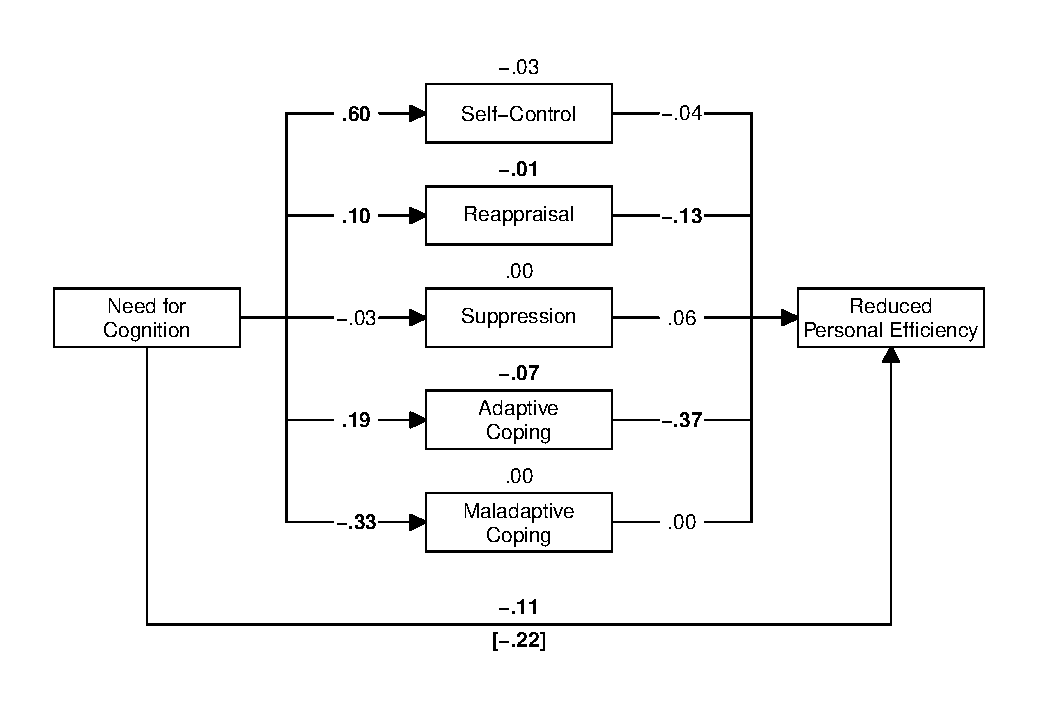
\includegraphics[keepaspectratio]{NFC-Caregiver_figures/Fig1.eps}}
\caption{Multiple mediation of the relationship between Need for Cognition with the burnout dimension reduced personal efficiency. Standardized coefficients are given (bold: \(p<.05\)). Indirect paths are provided above the mediators, the remaining direct effect is given at the bottom of the figure together with the total effect (in brackets).}
\end{figure}

\begin{table}[tbp]

\begin{center}
\begin{threeparttable}

\caption{\label{tab:RQ5}Mediation of the effect of Need for Cognition (NFC) on emotional exhaustion (EE)}

\footnotesize{

\begin{tabular}{lrrrrrr}
\toprule
 & \multicolumn{1}{c}{$B$} & \multicolumn{1}{c}{$SE$} & \multicolumn{1}{c}{$LB$} & \multicolumn{1}{c}{$UB$} & \multicolumn{1}{c}{$p$} & \multicolumn{1}{c}{$\beta$}\\
\midrule
\textit{Direct effect of NFC on EE} & -0.046 & 0.026 & -0.096 & 0.005 & .078 & -.088\\ \midrule
\textit{NFC to Mediators} &  &  &  &  &  & \\
\ \ \ a1: Self-Control & 0.277 & 0.015 & 0.247 & 0.307 & < .001 & .600\\
\ \ \ a2: Reappraisal & 0.040 & 0.016 & 0.009 & 0.071 & .012 & .104\\
\ \ \ a3: Suppression & -0.011 & 0.013 & -0.036 & 0.015 & .412 & -.034\\
\ \ \ a4: Adaptive Coping & 0.074 & 0.015 & 0.045 & 0.103 & < .001 & .194\\
\ \ \ a5: Maladaptive Coping & -0.042 & 0.005 & -0.052 & -0.033 & < .001 & -.330\\ \midrule
\textit{Mediators to EE} &  &  &  &  &  & \\
\ \ \ b1: Self-Control & -0.039 & 0.055 & -0.146 & 0.068 & .476 & -.035\\
\ \ \ b2: Reappraisal & -0.009 & 0.054 & -0.114 & 0.097 & .871 & -.006\\
\ \ \ b3: Suppression & 0.134 & 0.064 & 0.010 & 0.259 & .035 & .081\\
\ \ \ b4: Adaptive Coping & -0.417 & 0.055 & -0.526 & -0.308 & < .001 & -.306\\
\ \ \ b5: Maladaptive Coping & 0.597 & 0.166 & 0.271 & 0.923 & < .001 & .148\\ \midrule
\textit{Indirect effects} &  &  &  &  &  & \\
\ \ \ ind1: Self-Control & -0.011 & 0.015 & -0.041 & 0.019 & .477 & -.021\\
\ \ \ ind2: Reappraisal & 0.000 & 0.002 & -0.005 & 0.004 & .872 & -.001\\
\ \ \ ind3: Suppression & -0.001 & 0.002 & -0.005 & 0.002 & .452 & -.003\\
\ \ \ ind4: Adaptive Coping & -0.031 & 0.007 & -0.045 & -0.017 & < .001 & -.059\\
\ \ \ ind5: Maladaptive Coping & -0.025 & 0.008 & -0.041 & -0.010 & .001 & -.049\\ \midrule
\textit{Total effect} & -0.114 & 0.020 & -0.154 & -0.075 & < .001 & -.220\\
\bottomrule
\addlinespace
\end{tabular}

}

\begin{tablenotes}[para]
\normalsize{\textit{Note.} $N=642$. $B$ = unstandardized coefficient, $SE$ = standard error of $B$, $LB/UB$ = lower and upper bound of the 95\% confidence interval, $p$ = $p$-value, $\beta$ = standardized coefficient, a = paths from predictor to mediator, b = paths from mediator to outcome, ind = indirect effects a*b.}
\end{tablenotes}

\end{threeparttable}
\end{center}

\end{table}

\subsubsection{Research Question 5}\label{research-question-5}

Figure 2 and Table 3 show the model for \emph{emotional exhaustion}. Less than half of the total effect, \(\beta=\) -.22, \(p\) \textless{} .001, was due to the direct path, \(\beta=\) -.09, \(p\) = .078. Mediation occurred for adaptive coping, \(\beta=\) -.06, \(p\) \textless{} .001, and maladaptive coping, \(\beta=\) -.05, \(p\) = .001, but not for self-control, \(\beta=\) -.02, \(p\) = .477, reappraisal, \(\beta=\) .00, \(p\) = .872, or suppression, \(\beta=\) .00, \(p\) = .452.

\begin{figure}
\centering
\pandocbounded{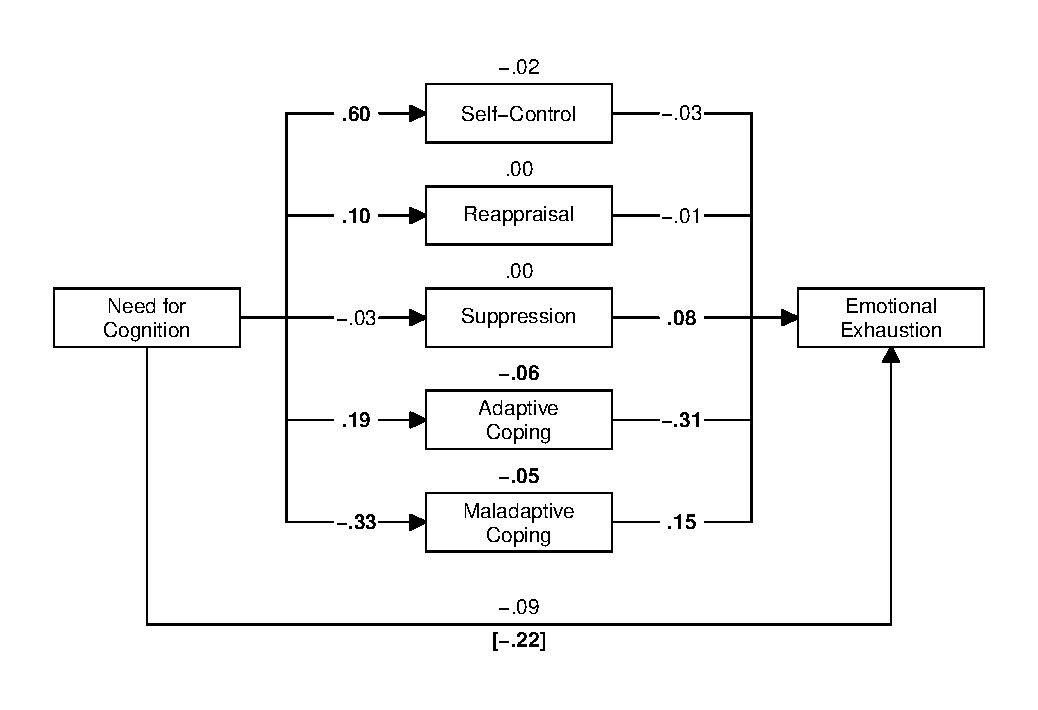
\includegraphics[keepaspectratio]{NFC-Caregiver_figures/Fig2.eps}}
\caption{Multiple mediation of the relationship between Need for Cognition with the burnout dimension emotional exhaustion. Standardized coefficients are given (bold: \(p< .05\)). Indirect paths are provided above the mediators, the remaining direct effect is given at the bottom of the figure together with the total effect (in brackets).}
\end{figure}

\begin{table}[tbp]

\begin{center}
\begin{threeparttable}

\caption{\label{tab:RQ6}Mediation of the effect of Need for Cognition (NFC) on depersonalization (DE)}

\footnotesize{

\begin{tabular}{lrrrrrr}
\toprule
 & \multicolumn{1}{c}{$B$} & \multicolumn{1}{c}{$SE$} & \multicolumn{1}{c}{$LB$} & \multicolumn{1}{c}{$UB$} & \multicolumn{1}{c}{$p$} & \multicolumn{1}{c}{$\beta$}\\
\midrule
\textit{Direct effect of NFC on DE} & -0.009 & 0.013 & -0.035 & 0.017 & .493 & -.034\\ \midrule
\textit{NFC to Mediators} &  &  &  &  &  & \\
\ \ \ a1: Self-Control & 0.277 & 0.015 & 0.247 & 0.307 & < .001 & .600\\
\ \ \ a2: Reappraisal & 0.040 & 0.016 & 0.009 & 0.071 & .012 & .104\\
\ \ \ a3: Suppression & -0.011 & 0.013 & -0.036 & 0.015 & .412 & -.034\\
\ \ \ a4: Adaptive Coping & 0.074 & 0.015 & 0.045 & 0.103 & < .001 & .194\\
\ \ \ a5: Maladaptive Coping & -0.042 & 0.005 & -0.052 & -0.033 & < .001 & -.330\\ \midrule
\textit{Mediators to DE} &  &  &  &  &  & \\
\ \ \ b1: Self-Control & -0.001 & 0.030 & -0.061 & 0.058 & .964 & -.002\\
\ \ \ b2: Reappraisal & -0.067 & 0.027 & -0.121 & -0.013 & .015 & -.095\\
\ \ \ b3: Suppression & 0.179 & 0.031 & 0.117 & 0.241 & < .001 & .210\\
\ \ \ b4: Adaptive Coping & -0.134 & 0.029 & -0.191 & -0.077 & < .001 & -.190\\
\ \ \ b5: Maladaptive Coping & 0.221 & 0.080 & 0.064 & 0.379 & .006 & .106\\ \midrule
\textit{Indirect effects} &  &  &  &  &  & \\
\ \ \ ind1: Self-Control & 0.000 & 0.008 & -0.017 & 0.016 & .964 & -.001\\
\ \ \ ind2: Reappraisal & -0.003 & 0.001 & -0.005 & 0.000 & .065 & -.010\\
\ \ \ ind3: Suppression & -0.002 & 0.002 & -0.006 & 0.003 & .420 & -.007\\
\ \ \ ind4: Adaptive Coping & -0.010 & 0.003 & -0.015 & -0.004 & < .001 & -.037\\
\ \ \ ind5: Maladaptive Coping & -0.009 & 0.004 & -0.017 & -0.002 & .010 & -.035\\ \midrule
\textit{Total effect} & -0.033 & 0.010 & -0.052 & -0.014 & .001 & -.124\\
\bottomrule
\addlinespace
\end{tabular}

}

\begin{tablenotes}[para]
\normalsize{\textit{Note.} $N=642$. $B$ = unstandardized coefficient, $SE$ = standard error of $B$, $LB/UB$ = lower and upper bound of the 95\% confidence interval, $p$ = $p$-value, $\beta$ = standardized coefficient, a = paths from predictor to mediator, b = paths from mediator to outcome, ind = indirect effects a*b.}
\end{tablenotes}

\end{threeparttable}
\end{center}

\end{table}

\subsubsection{Research Question 6}\label{research-question-6}

Figure 3 and Table 4 show the model for \emph{depersonalization}. About one third of the total effect, \(\beta=\) -.12, \(p\) \textless{} .001, reflected the direct path, \(\beta=\) -.03, \(p\) = .493. Again, mediation was found for adaptive and maladaptive coping, \(\beta=\) -.04, \(p\) \textless{} .001, and \(\beta=\) -.03, \(p\) = .010, but not for self-control, \(\beta=\) .00, \(p\) = .964, reappraisal, \(\beta=\) -.01, \(p\) = .065, or suppression, \(\beta=\) -.01, \(p\) = .420.

\begin{figure}
\centering
\pandocbounded{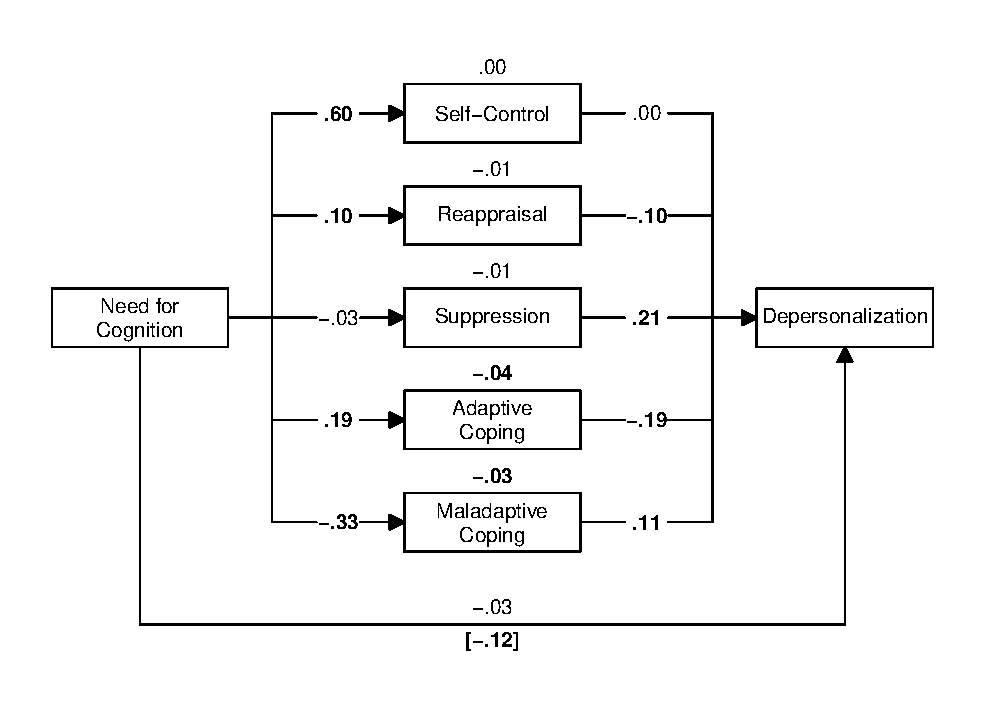
\includegraphics[keepaspectratio]{NFC-Caregiver_figures/Fig3.eps}}
\caption{Multiple mediation of the relationship between Need for Cognition with the burnout dimension depersonalization. Standardized coefficients are given (bold: \(p< .05\)). Indirect paths are provided above the mediators, the remaining direct effect is given at the bottom of the figure together with the total effect (in brackets).}
\end{figure}

\section{Discussion}\label{discussion}

\ldots{}

\newpage

\section{References}\label{references}

\phantomsection\label{refs}
\begin{CSLReferences}{1}{0}
\bibitem[\citeproctext]{ref-Abler-2009}
Abler, B., \& Kessler, H. (2009). {Emotion Regulation Questionnaire -- Eine deutschsprachige Fassung des ERQ von Gross und John}. \emph{Diagnostica}, \emph{55}(3), 144--152. \url{https://doi.org/10.1026/0012-1924.55.3.144}

\bibitem[\citeproctext]{ref-R-papaja}
Aust, F., \& Barth, M. (2024). \emph{{papaja}: {Prepare} reproducible {APA} journal articles with {R Markdown}}. \url{https://doi.org/10.32614/CRAN.package.papaja}

\bibitem[\citeproctext]{ref-R-tinylabels}
Barth, M. (2025). \emph{{tinylabels}: Lightweight variable labels}. \url{https://doi.org/10.32614/CRAN.package.tinylabels}

\bibitem[\citeproctext]{ref-Bertrams-2009}
Bertrams, A., \& Dickhäuser, O. (2009). {Messung dispositioneller Selbstkontroll-Kapazität}. \emph{Diagnostica}, \emph{55}(1), 2--10. \url{https://doi.org/10.1026/0012-1924.55.1.2}

\bibitem[\citeproctext]{ref-Bianchi-2015}
Bianchi, R., Schonfeld, I. S., \& Laurent, E. (2015). Burnout--depression overlap: A review. \emph{Clinical Psychology Review}, \emph{36}, 28--41. \url{https://doi.org/10.1016/j.cpr.2015.01.004}

\bibitem[\citeproctext]{ref-Bless-1994}
Bless, H., Wänke, M., Bohner, G., Fellhauer, R. F., \& Schwarz, N. (1994). Need for cognition: Eine skala zur erfassung von engagement und freude bei denkaufgaben. \emph{Zeitschrift Für Sozialpsychologie}, \emph{25}, 147--154. \url{https://pub.uni-bielefeld.de/publication/1779110}

\bibitem[\citeproctext]{ref-Buessing-1992}
Büssing, A., \& Perrar, K.-M. (1992). Die {Messung von Burnout. Untersuchung einer deutschen Fassung des Maslach Burnout Inventory (MBI-D)}. \emph{Diagnostica}, \emph{38}, 328--353.

\bibitem[\citeproctext]{ref-Dewa-2017}
Dewa, C. S., Loong, D., Bonato, S., \& Trojanowski, L. (2017). The relationship between physician burnout and quality of healthcare in terms of safety and acceptability: A systematic review. \emph{BMJ Open}, \emph{7}(6), e015141. \url{https://doi.org/10.1136/bmjopen-2016-015141}

\bibitem[\citeproctext]{ref-Faul-2007}
Faul, F., Erdfelder, E., Lang, A., \& Buchner, A. (2007). \emph{G*power (3.1.9.7) {[}software{]}}. \url{http://www.gpower.hhu.de/}

\bibitem[\citeproctext]{ref-Galanis-2021}
Galanis, P., Vraka, I., Fragkou, D., Bilali, A., \& Kaitelidou, D. (2021). Nurses' burnout and associated risk factors during the COVID-19 pandemic: A systematic review and meta-analysis. \emph{Journal of Advanced Nursing}. \url{https://doi.org/10.1111/jan.14839}

\bibitem[\citeproctext]{ref-Gignac-2016}
Gignac, G. E., \& Szodorai, E. T. (2016). Effect size guidelines for individual differences researchers. \emph{Personality and Individual Differences}, \emph{102}, 74--78. \url{https://doi.org/10.1016/j.paid.2016.06.069}

\bibitem[\citeproctext]{ref-Grass-2018}
Grass, J., John, N., \& Strobel, A. (2018). Freude am denken als schlüssel zum erfolg? Die bedeutung von need for cognition für subjektives erleben und leistung im studium. \emph{Zeitschrift Für Pädagogische Psychologie}, \emph{32}(3), 145--154. \url{https://doi.org/10.1024/1010-0652/a000222}

\bibitem[\citeproctext]{ref-Kadur-2018}
Kadur, A. M. (2018). \emph{{Risiko}- und {Protektivfaktoren} der {Persönlichkeit} von {Pflegekräften} ({Unpublished Master's Thesis})}. Chemnitz University of Technology.

\bibitem[\citeproctext]{ref-Maslach-1998}
Maslach, C. (1998). A multidimensional theory of burnout. In C. L. Cooper (Ed.), \emph{Theories of organizational stress} (pp. 68--85). Oxford University Press. \url{https://www.researchgate.net/profile/Christina-Maslach/publication/280939428_A_Multidimensional_Theory_of_Burnout/links/55cd2b0708aebebb8f577ea5/A-Multidimensional-Theory-of-Burnout.pdf}

\bibitem[\citeproctext]{ref-Maslach-2003}
Maslach, C. (2003). Job burnout: New directions in research and intervention. \emph{Current Directions in Psychological Science}, \emph{12}(5), 189--192. https://doi.org/\url{https://doi.org/10.1111/1467-8721.01258}

\bibitem[\citeproctext]{ref-R-here}
Müller, K. (2020). \emph{Here: A simpler way to find your files}. \url{https://CRAN.R-project.org/package=here}

\bibitem[\citeproctext]{ref-Oreskovich-2012}
Oreskovich, M. R., Kaups, K. L., Balch, C. M., Hanks, J. B., Satele, D., Sloan, J. A., Meredith, C. W., Buhl, A., Dyrbye, L. N., \& Shanafelt, T. D. (2012). Prevalence of alcohol use disorders among american surgeons. \emph{Archives of Surgery}, \emph{147}(2), 168--175. \url{https://doi.org/10.1001/archsurg.2011.1481}

\bibitem[\citeproctext]{ref-Parandeh-2022}
Parandeh, A., Ashtari, S., Rahimi-Bashar, F., Gohari-Moghadam, K., \& Vahedian-Azimi, A. (2022). Prevalence of burnout among health care workers during coronavirus disease ({COVID-19}) pandemic: A systematic review and meta-analysis. \emph{Professional Psychology: Research and Practice}, \emph{53}, 564--573. \url{https://doi.org/10.1037/pro0000483}

\bibitem[\citeproctext]{ref-R-RStudio}
Posit Team. (2024). \emph{RStudio: Integrated development environment for r}. Posit Software, PBC. \url{http://www.posit.co/}

\bibitem[\citeproctext]{ref-Prasad-2021}
Prasad, K., McLoughlin, C., Stillman, M., Poplau, S., Goelz, E., Taylor, S., Nankivil, N., Brown, R., Linzer, M., Cappelucci, K., Barbouche, M., \& Sinsky, C. A. (2021). Prevalence and correlates of stress and burnout among u. S. Healthcare workers during the COVID-19 pandemic: A national cross-sectional survey study. \emph{EClinicalMedicine}, \emph{35}, 100879. \url{https://doi.org/10.1016/j.eclinm.2021.100879}

\bibitem[\citeproctext]{ref-Questback-2017}
Questback. (2017). \emph{EFS survey {[}software{]}}. \url{https://www.questback.com/de}

\bibitem[\citeproctext]{ref-R-base}
R Core Team. (2024). \emph{R: A language and environment for statistical computing}. R Foundation for Statistical Computing. \url{https://www.R-project.org/}

\bibitem[\citeproctext]{ref-R-psych}
Revelle, W. (2024). \emph{Psych: Procedures for psychological, psychometric, and personality research}. Northwestern University. \url{https://CRAN.R-project.org/package=psych}

\bibitem[\citeproctext]{ref-Rink-2023}
Rink, L. C., Oyesanya, T. O., Adair, K. C., Humphreys, J. C., Silva, S. G., \& Sexton, J. B. (2023). Stressors among healthcare workers: A summative content analysis. \emph{Global Qualitative Nursing Research}, \emph{10}, 1--13. \url{https://doi.org/10.1177/23333936231161127}

\bibitem[\citeproctext]{ref-R-lavaan}
Rosseel, Y. (2012). {lavaan}: An {R} package for structural equation modeling. \emph{Journal of Statistical Software}, \emph{48}(2), 1--36. \url{https://doi.org/10.18637/jss.v048.i02}

\bibitem[\citeproctext]{ref-Satow-2012}
Satow, L. (2012). \emph{{Stress- und Coping-Inventar (SCI): Test- und Skalendokumentation}}. \url{https://www.drsatow.de/tests/stress-und-coping-inventar/}

\bibitem[\citeproctext]{ref-Shanafelt-2009}
Shanafelt, T. D., Balch, C. M., Bechamps, G., Russell, T. P., Dyrbye, L. N., Satele, D., Collicott, P., Novotny, P. J., Sloan, J. A., \& Freischlag, J. A. (2009). Burnout and career satisfaction among american surgeons. \emph{Annals of Surgery}, \emph{250}(3), 463--471. \url{https://doi.org/10.1097/sla.0b013e3181ac4dfd}

\bibitem[\citeproctext]{ref-Shanafelt-2011}
Shanafelt, T. D., Balch, C. M., Dyrbye, L. N., Bechamps, G., Russell, T., Satele, D., Rummans, T. A., Swartz, K., Novotny, P. J., Sloan, J. A., \& Oreskovich, M. R. (2011). Special report: Suicidal ideation among american surgeons. \emph{Archives of Surgery}, \emph{146}(1), 54--62. \url{https://doi.org/10.1001/archsurg.2010.292}

\bibitem[\citeproctext]{ref-Simmons-2012}
Simmons, J. P., Nelson, L. D., \& Simonsohn, U. (2012). \emph{A 21 word solution}. \url{https://doi.org/10.2139/ssrn.2160588}

\bibitem[\citeproctext]{ref-R-shape}
Soetaert, K. (2024). \emph{Shape: Functions for plotting graphical shapes, colors}. \url{https://doi.org/10.32614/CRAN.package.shape}

\bibitem[\citeproctext]{ref-West-2018}
West, C., Dyrbye, L. N., \& Shanafelt, T. D. (2018). Physician burnout: Contributors, consequences and solutions. \emph{Journal of Internal Medicine}, \emph{283}(6), 516--529. \url{https://doi.org/10.1111/joim.12752}

\bibitem[\citeproctext]{ref-R-dplyr}
Wickham, H., François, R., Henry, L., Müller, K., \& Vaughan, D. (2023). \emph{Dplyr: A grammar of data manipulation}. \url{https://doi.org/10.32614/CRAN.package.dplyr}

\bibitem[\citeproctext]{ref-Zerna-2022}
Zerna, J., Engelmann, N., Strobel, A., \& Strobel, A. (2022). Need for cognition and burnout in teachers -- a replication and extension study. \emph{Health Psychology Open}, \emph{9}(2), 2055102922113. \url{https://doi.org/10.1177/20551029221139679}

\bibitem[\citeproctext]{ref-Ziessler-2019}
Ziessler, K. (2019). \emph{{Need for Cognition als Ressource für helfende Berufe} ({Unpublished Bachelor's Thesis})}. Chemnitz University of Technology.

\end{CSLReferences}


\end{document}
